\providecommand{\setflag}{\newif \ifwhole \wholefalse}
\setflag
\ifwhole\else

% Typography and geometry ----------------------------------------------------
\documentclass[letterpaper]{scrbook}
\usepackage[inner=3cm,top=2.5cm,outer=3.5cm]{geometry}

\renewcommand\familydefault{bch}
\usepackage[utf8]{inputenc}
\usepackage{microtype}
\usepackage[small]{caption}
\usepackage[small]{titlesec}
\raggedbottom

% Graphics -------------------------------------------------------------------
\usepackage[pdftex]{graphicx}
\graphicspath{{_include/}}
\DeclareGraphicsExtensions{.png,.pdf}

% Code formatting ------------------------------------------------------------
\usepackage{fancyvrb}
\usepackage{courier}
\usepackage{listings}
\usepackage{color}
\usepackage{alltt}


\definecolor{comment}{rgb}{0.60, 0.60, 0.53}
\definecolor{background}{rgb}{0.97, 0.97, 1.00}
\definecolor{string}{rgb}{0.863, 0.066, 0.266}
\definecolor{number}{rgb}{0.0, 0.6, 0.6}
\definecolor{variable}{rgb}{0.00, 0.52, 0.70}
\lstset{
  basicstyle=\ttfamily,
  keywordstyle=\bfseries, 
  identifierstyle=,  
  commentstyle=\color{comment} \emph,
  stringstyle=\color{string},
  showstringspaces=false,
  columns = fullflexible,
  backgroundcolor=\color{background},
  mathescape = true,
  escapeinside=&&,
  fancyvrb
}
\newcommand{\code}[1]{\lstinline!#1!}
\newcommand{\f}[1]{\lstinline!#1()!}



% Links ----------------------------------------------------------------------

\usepackage{hyperref}
\definecolor{slateblue}{rgb}{0.07,0.07,0.488}
\hypersetup{colorlinks=true,linkcolor=slateblue,anchorcolor=slateblue,citecolor=slateblue,filecolor=slateblue,urlcolor=slateblue,bookmarksnumbered=true,pdfview=FitB}
\usepackage{url}

% Tables ---------------------------------------------------------------------
\usepackage{longtable}
\usepackage{booktabs}

% Miscellaneous --------------------------------------------------------------
\usepackage{pdfsync}
\usepackage{appendix}

\usepackage[round,sort&compress,sectionbib]{natbib}
\bibliographystyle{plainnat}


\title{ggplot2}
\author{Hadley Wickham}

\begin{document}
\fi


% SET_DEFAULTS
%   GG-WIDTH: 4  GG-HEIGHT: 4
%   TEX-WIDTH: 0.5\linewidth
%   INLINE: FALSE
% 

% END


\chapter{Manipulating plot rendering with \code{grid}}
\label{cha:grid}

\section{Introduction}

% The are two ways to do this: common options are exposed by the {\tt ggopt} function, or you can use the grid package to modify the graphical output of ggplot.  The few options provided by {\tt ggopt} allow you to easily modify the most commonly tweaked parts of ggplot graphics, but for more control you can use the power of grid to delve into the dark depths of {\tt ggplot} and tweak to your heart's content.

% TODO: MORE BACKGROUND!

What is \pkg{grid}?  It's the graphics engine that powers ggplot.  It is responsible for drawing the graphic object onto the screen or saving it to a graphics file.  It provides a system of viewports, which define regions on the plot, and a comprehensive set of units for describing size and position. This chapter can not hope to provide a comprehensive introduction to grid, but should hopefully provide enough examples to get you going.   I highly recommend the book ``R Graphics'' \citep{murrell:2005}, by the author of grid,  as a companion to this chapter.  If you can't get the book, at least read Chapter 5, ``The grid graphics model'', which is available online for free at  \url{http://www.stat.auckland.ac.nz/~paul/RGraphics/chapter5.pdf}.

The grobs (graphical objects) used in this chapter are a bit different to the geoms (geometric objects) used in previous chapters.  A grob is the object that is actually drawn onto the screen, while a geom is a more abstract object which describes the type of object used to draw a plot.  An example may make this more clear. In a line plot, the geom describes that the data should be visualised with a line, and the grobs draw the line itself, as well as the other lines that appear in the grid and axes.

The chapter begins with a discussion of the structure of viewports (\secref{sec:plot-viewports}) and grobs (\secref{sec:plot-grobs}) used by \ggplot, and then continues to describe the four principle ways to enhance a plot with grid:

\begin{itemize}
  \item Custom element functions
  \item Edit existing objects on the plot, \secref{sec:grid-existing}.
  \item Add annotations to the plot, \secref{sec:grid-new}.
  \item Removing grobs from a plot, \secref{sec:grid-delete}.
  \item Arrange multiple plots on a single page, \secref{sec:grid-layout}.
\end{itemize}

\section{Plot viewports}
\label{sec:plot-viewports}

Viewports define the basic regions of the plot.  The structure will vary slightly from plot to plot, depending on the type of faceting used, but the basics will remain the same. 

The {\tt panels} viewport contains the meat of the plot: strip labels, axes and faceted panels.  The viewports are named according to both their job and their position on the plot.  A prefix (listed below) describes the contents of the viewport, and is followed by integer x and y position (counting from bottom left) separated by ``\_''.  Figure~\ref{fig:panelvp} illustrates this naming scheme for a 2$\times$2 plot.

\begin{itemize}
  \item {\tt strip\_h}: horizontal strip labels
  \item {\tt strip\_v}: vertical strip labels
  \item {\tt axis\_h}: horizontal axes
  \item {\tt axis\_v}: vertical axes
  \item {\tt panel}: faceting panels
\end{itemize}

\begin{figure}[htbp]
  \centering
    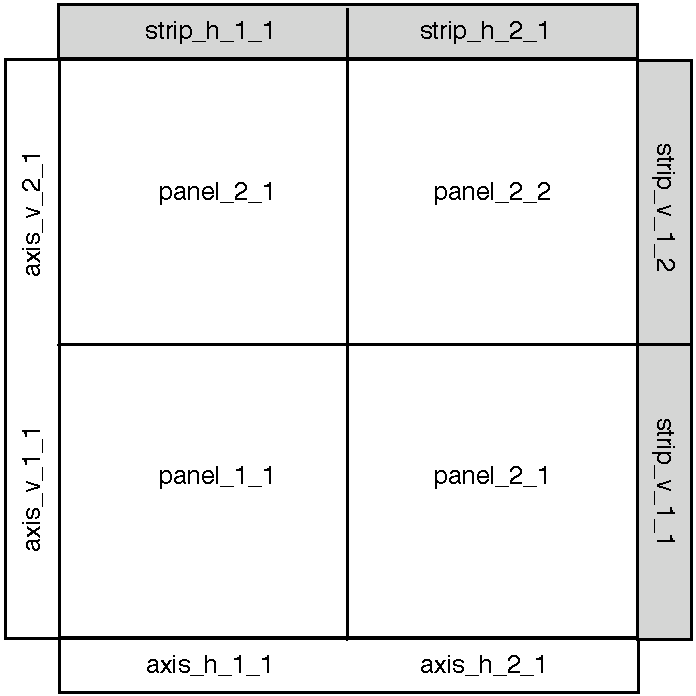
\includegraphics[width=0.5 \linewidth]{grid-panelvp}
  \caption{Naming scheming of the panel viewports}
  \label{fig:panelvp}
\end{figure}

The \code{panels} viewport is contained inside the \code{background} viewport which also contains the following viewports:

\begin{itemize}
  \item \code{title}, \code{xlabel}, and \code{ylabel}: for the plot title, and x and y axis labels
  \item \code{legend_box}: for all of the legends for the plot
\end{itemize}

\noindent Figure~\ref{fig:viewports} labels a plot with a representative sample of these viewports.  To get a list of all viewports on the current plot, run \code{current.vpTree(all=TRUE)}.

\begin{figure}[htbp]
  \centering
    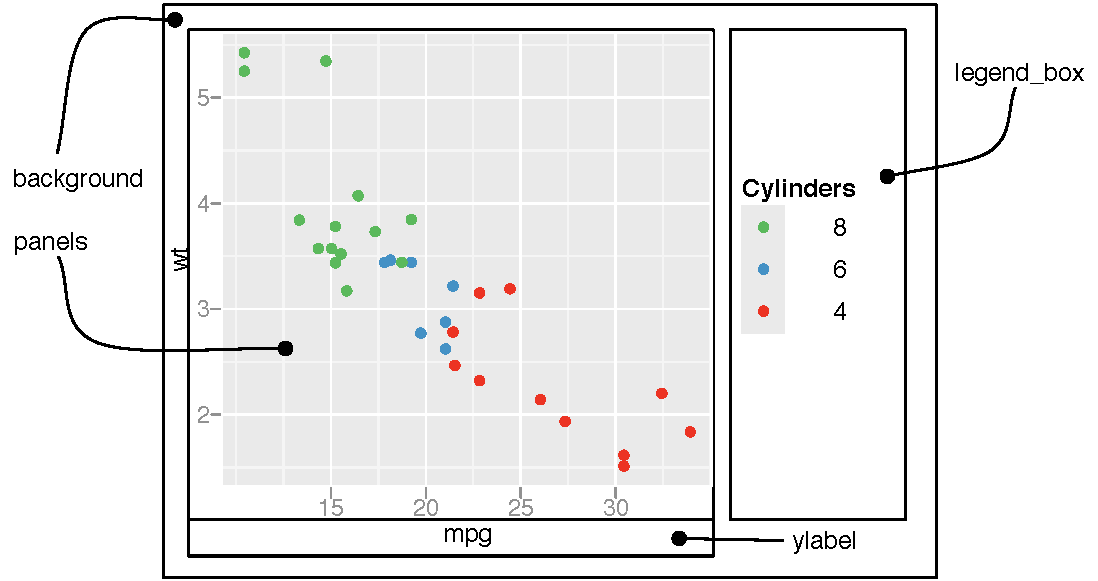
\includegraphics[width=\linewidth]{grid-viewports}
  \caption{Diagram showing the structure and names of viewports.}
  \label{fig:viewports}
\end{figure}

\section{Plot grobs}
\label{sec:plot-grobs}

Grob names have three components: the name of the grob, the class of the grob, and a unique numeric suffix.  The three components are joined together with ``.'' to give a name like {\tt title.text.435} or {\tt ticks.segments.15}.  These three components ensure that all grob names are unique, and allow you to select multiple grobs with the same name at the same time.

You can see a list of all the grobs in the current plot with {\tt grid.ls()}.  Here's an example after drawing the a simple plot:

\begin{alltt}
GRID.gTree.4189
  plot.background.rect.4188
  plot.title.text.4182
  axis.title.x.text.4184
  axis.title.y.text.4186
  plot.gTree.4180
    panel.gTree.4170
      grill.gTree.4168
        panel.background.rect.4159
        panel.grid.minor.y.polyline.4161
        panel.grid.minor.x.polyline.4163
        panel.grid.major.y.polyline.4165
        panel.grid.major.x.polyline.4167
      GRID.gTree.4131
        geom_point.points.4130
    axis_v.absoluteGrob.4171
      axis.ticks.segments.4142
      axis.text.y.text.4139
    axis_v.nullGrob.4172
    axis_h.absoluteGrob.4175
      axis.ticks.segments.4136
      axis.text.x.text.4133
\end{alltt}

Figure~\ref{fig:grobs} labels some of these grobs.  The grobs are arranged hierarchically, but it's hard to capture this in a diagram.

\begin{figure}[htbp]
  \centering
    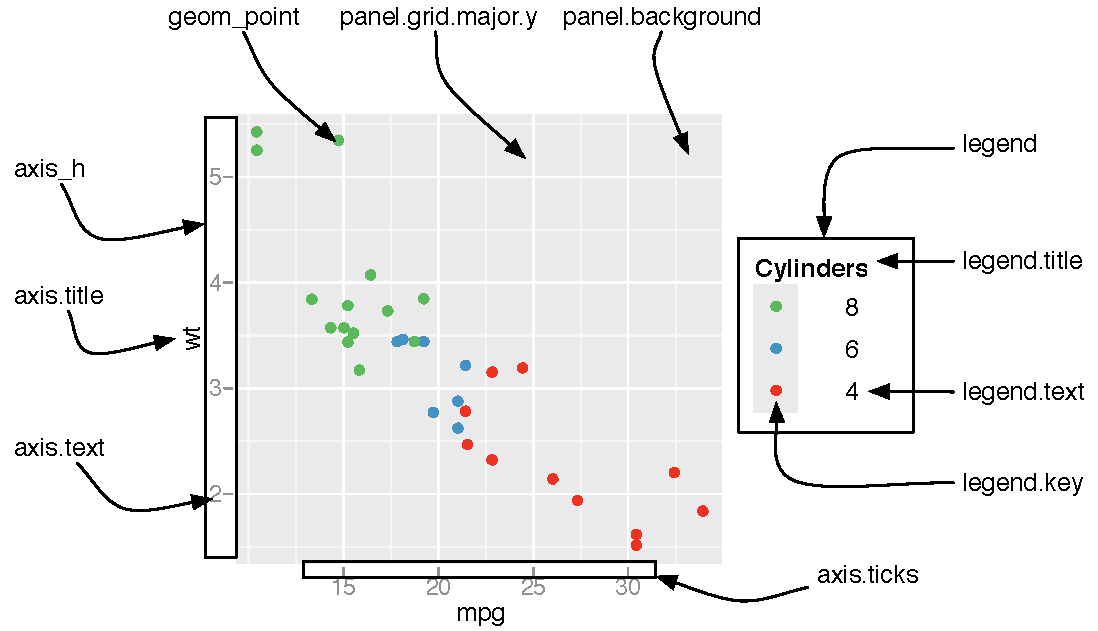
\includegraphics[width=\linewidth]{grid-grobs}
  \caption{A selection of the most important grobs.  \code{geom_point}, \code{major-vertical} and \code{label} point to a single element of the grob.}
  \label{fig:grobs}
\end{figure}

The most important components are:

\begin{itemize}
  \item The geom displayed in the plot: {\tt geom\_point}.

  \item {\tt xaxis} and {\tt yaxis}, the axes, containing {\tt labels} and {\tt ticks}.

  \item Axis labels and title: {\tt xlabel}, {\tt ylabel}, {\tt title}.

  \item {\tt guide}, the internal guides within a panel (background, and grid lines)

\end{itemize}

\section{Custom element functions}
\label{sec:custom-elements}

To see how to write custom element functions, it's good to start by seeing how the built-in element functions work:

% INTERWEAVE
% 
% str(args(theme_text()))
% str(args(theme_rect()))
% str(args(theme_line()))
\input{_include/1d9a99fa7a894d2c4a76f7c03cb0fea2.tex}
% END

You'll notice that these are very similar to the arguments to \f{textGrob}, \f{rectGrob} and \f{polylineGrob} and these are exactly the functions that they are based on.  All that the element function do is set up some defaults.  

If you want to write your own, you need to copy this basic idea: take position arguments, and return a grid grob.  For example, let's say we'd like to give the strips a 3d appearance.  We can do this by drawing a rectangle, and then drawing highlights on the top-right and low-lights (shadows) on the bottom-left.


\section{Editing existing objects on the plot}
\label{sec:grid-existing}

From time to time, the theming system will not give you enough control.  This may occur if you want to modify a single element of a plot, like one grid line or a single label.  Where possible, using the theming system will be easier, because using grid will affect a component, but not the space saved for that element.

Most of the difficulty in modifying elements of the plot is figuring out what the grob you want to modify is called.  Once you have that you can use {\tt grid.gedit}, to locate and then modify that grob. 

To fully identify a grob, you need to use a \code{gPath}.  A \code{gPath} can either be a string specifying a single grob name, or a sequence of grob names that describe hierarchy to travel down to get to the grob of interest with the {\tt gPath} function.  Using a string will find all grobs with that name regardless of their position in the hierarchy.  For example, {\tt "label"} will find all grobs called label, regardless of where they are.  To be more specific, using {\tt gPath("parent", "child")} will only find grobs named ``child'' with a parent called ``parent''.  For example, {\tt gPath("xaxis", "label")} will locate only labels on the x-axis.

Modifying a grob requires some knowledge of the different parameters of the grob.  This is where the second part of the grob name is useful, as it will tell you whether you are modifying a line, or a rect or a text grob.  You can get more information by looking at the documentation for that grob, eg. {\tt ?grid.rect, ?grid.text, ?grid.lines}   As well as individual parameters, all grobs share a common set of graphical parameters described in Table \ref{tbl:gpar}. Appendix~\ref{cha:specifications} describes the values that these may take.

\begin{table}
  \begin{center}
  \begin{tabular}{lll}
    \toprule
    Grid parameter & \ggplot aesthetic &  Description \\
    \midrule
    lwd & size & Line width (in pts) \\
    col & colour & Border colour \\
    fill  & fill & Fill colour \\
    fontsize & size & Font size (in pts) \\
    fontface & --- & Font face (bold, italic, ...) \\
    \bottomrule
  \end{tabular}
  \end{center}
  \caption{Common graphical parameters for grid grobs.  Note that point size is controlled separately.}
  \label{tbl:gpar}
\end{table}

In this example, we edit the font of all labels.

\begin{alltt}
qplot(mpg, wt, data = mtcars, facets = . ~ cyl)
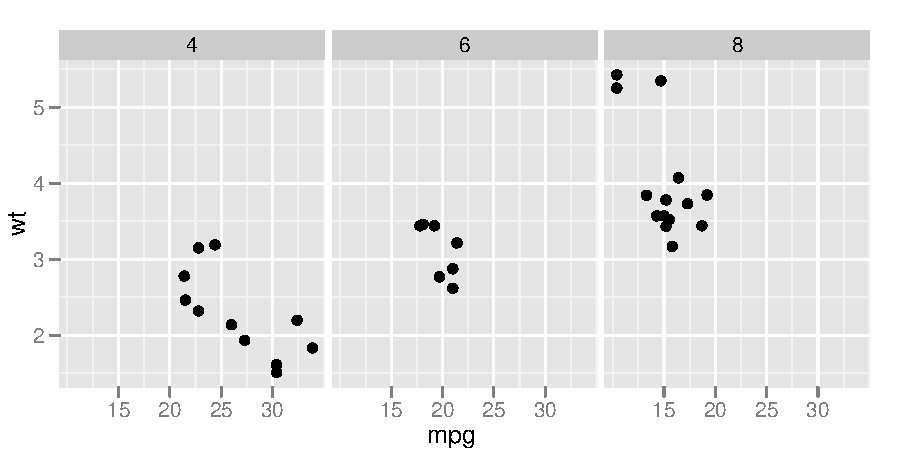
\includegraphics[width=0.75\linewidth]{grid1}
grid.gedit("text", gp = gpar(fontsize=14, col="red"))
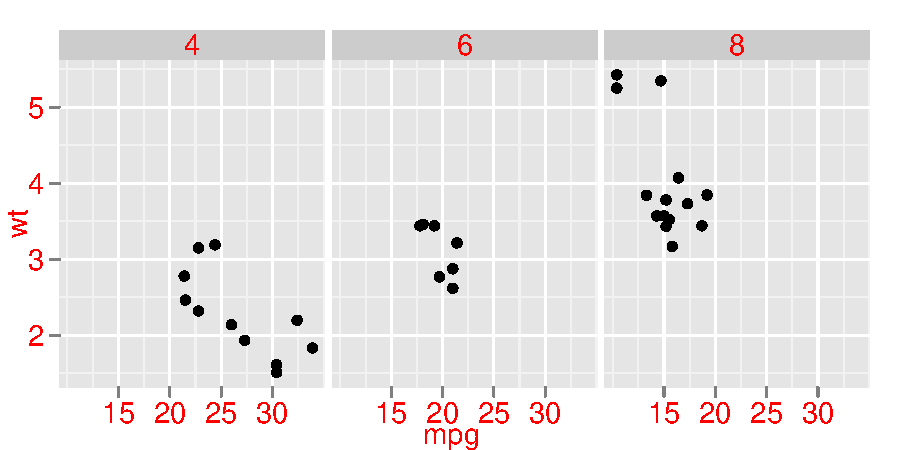
\includegraphics[width=0.75\linewidth]{grid2}
\end{alltt}
% dev.copy2pdf(file = "grid1.pdf", width = 6, height = 3)
% dev.copy2pdf(file = "grid2.pdf", width = 6, height = 3)

To edit just one type of label, we need to use the hierarchy of grobs and the {\tt gPath} function:

\begin{alltt}
qplot(mpg, wt, data = mtcars, facets = . ~ cyl)
grid.gedit(gPath("strip","text"), gp = gpar(fontface="bold"))
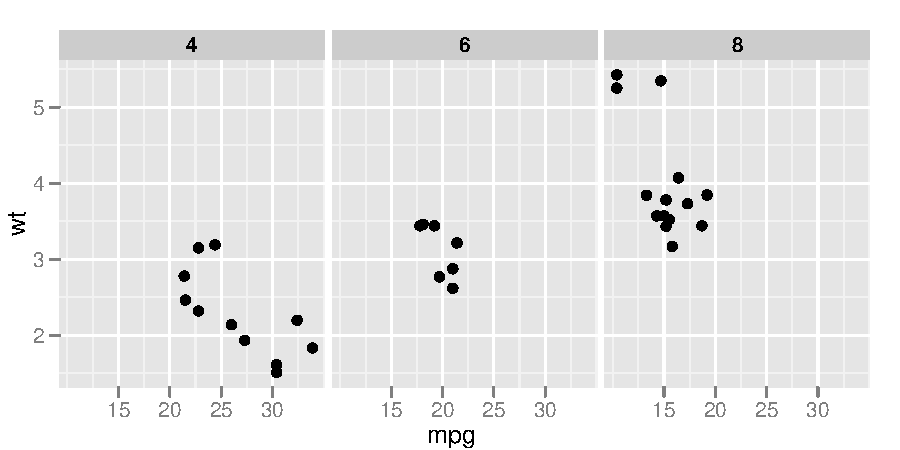
\includegraphics[width=0.75\linewidth]{grid3}
grid.gedit(gPath("axis_h", "text"), gp = gpar(col="red"))
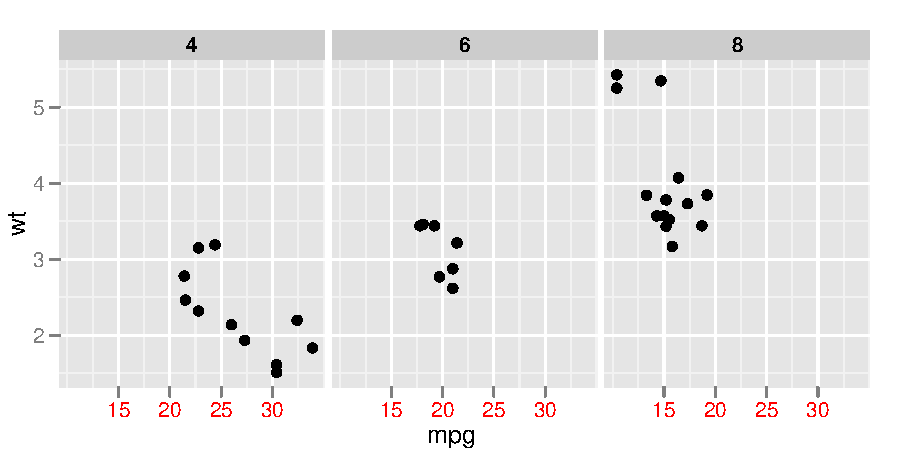
\includegraphics[width=0.75\linewidth]{grid4}
\end{alltt}
% dev.copy2pdf(file = "grid3.pdf", width = 6, height = 3)
% dev.copy2pdf(file = "grid4.pdf", width = 6, height = 3)

\section{Removing grobs}
\label{sec:grid-delete}

You can use \f{grid.remove} to completely remove a grob.  However, the space it takes up will remain there:

% LISTING
% 
% qplot(mpg, wt, data=mtcars, facets = . ~ cyl)
% grid.gremove(gPath("strip", "background"))
% grid.gremove(gPath("guide", "background"))
% grid.gremove("major")
% grid.gremove("axis")
\input{_include/b54778cc72cb3335dd92934f5c2f506b.tex}
% END

You can use an alternative method to remove top level viewports.  There are plot-level options \code{keep} and \code{drop}, which specify which viewports to keep or drop respectively.  For example:

% LISTING
% 
% p <- qplot(mpg, wt, data=mtcars, main = "My plot")
% p + opts(keep = "panel")
% p + opts(ignore = c("xlabel", "ylabel"))
\input{_include/bb6c56f6f3628cff036ae7f3f5055cbb.tex}
% END

\section{Adding annotations}\label{sec:adding_annotation}
\label{sec:grid-new}

Many annotations can be done with {\tt geom\_text}, {\tt geom\_abline}, {\tt geom\_vline} and {\tt geom\_hline}, so try those first.  If you need more flexibility you can add annotations with grid.  When you add annotations to a plot you need to specify where they will appear.  In grid this is described by a system of viewports.  Different viewports describe different regions of output on the plot, for example, the axes, the plotting region and the faceting strips.

To add annotations to a plot you have to specify the viewport when you add extra grobs.  For example:

% LISTING
% 
% qplot(wt, mpg, data=mtcars, colour=cyl)
% grid.circle(vp="layout::panel_1_1")
\input{_include/ea53669e9afc6f1641fff6e020ae7105.tex}
% END

Panel viewports will have a coordinate system set up for points, while x- and y- axes will only have one dimension defined.  For example, on the x-axis there will be native coordinates for the x-dimension, but not the y-dimension.

% LISTING 
% 
% qplot(wt, mpg, data=mtcars, colour=cyl)
% grid.lines(x = unit(c(0,1), "npc"), y = unit(23, "native"),
%    vp = "layout::panel_1_1")
% grid.lines(x = unit(c(0,1), "npc"), y = unit(23, "native"),
%    vp = "layout::axis_v_1_1")
\input{_include/59a12cde48d774fb117f3e7318006b19.tex}
% END

\section{Customising layout}
\label{sec:grid-layout}

By default, showing a {\tt ggplot} object at the R command prompt will display to the screen.  To exercise more control, there are two options you can set: \code{keep} and \code{drop}.  If you just want the plot (no labels, titles or legends) you can use \code{opts(keep = "panels")}:

% INTERWEAVE
% 
% p <- qplot(wt, mpg, data=mtcars, colour=cyl)
% p + opts(keep = "panels")
\input{_include/4b19280eab34f9514ea704d296bd7466.tex}
% END

By default, {\tt ggplot} always clears the screen and draws to the entire device.  You customise this in two ways. One way is to setup a viewport and push it on to the display, then draw the plot with {\tt newpage=FALSE}. {\tt pushViewport} adds the viewport to the list of viewports on the display.   Afterwards, {\tt upViewport} returns you to the viewport for the entire page, preparing you for the next set of output.

% LISTING
% 
% p <- qplot(wt, mpg, data=mtcars, colour=cyl)
% grid.newpage()
% pushViewport(viewport(height=0.4, width=0.4, x=0.4, y=0.8))
% print(p, newpage=FALSE, pretty=FALSE)
% upViewport()
\input{_include/896b229f927422d070198f97adefeaa2.tex}
% END

Alternatively, you can set up your own set of viewports, and then specify which one the plot should be drawn to.  Here we use {\tt upViewport} before displaying the plot so we are in the top level viewport before we start plotting.

% LISTING
% 
% grid.newpage()
% pushViewport(viewport(height = 0.5, width = 0.5, x = 0.5, y = 0.5, 
%   name="small", angle=40))
% upViewport()
% print(p, vp="small")
\input{_include/b7306e00b4d5e12d9578c2d50f8d5537.tex}
% END

Obviously, this is very useful if you want to layout plots in a complicated grid.  In this case, {\tt grid.layout} is very useful, as it allows you to set up a grid of viewports with arbitrary heights and widths.  You still need to create each viewport, but instead of explicitly specifying the position and size, you can specify the row and column of the layout.

% LISTING
% 
% p <- qplot(wt, mpg, data = mtcars, colour = cyl)
% 
% vplayout <- function(x, y) 
%   viewport(layout.pos.row = x, layout.pos.col = y)
% grid.newpage()
% pushViewport(viewport(layout = grid.layout(3,3)))
% 
% print(p, vp=vplayout(1,1))
% print(p, vp=vplayout(2:3,2:3))
% print(p, vp=vplayout(1, 2:3))
% print(p, vp=vplayout(2:3, 1))
\input{_include/4f19e0618407a42a5fa71eb184d43db3.tex}
% END

This is useful for arranging plots in a wider range of ways than what you can do with faceting.   You should be careful to ensure that scales are consistent over the different plots.  There is currently no easy way to do this, except to keep track of the maximum and minimum yourself, and then manually set the scales of the plot.

\section{Saving your work} 
\label{sec:grid-save}

Using \f{grid.gedit} works fine if you are editing the plot on screen, but if you want to save it to disk you need take some extra steps, or you will end up with multiple pages of output, each showing one change.  The key is not to modify the plot on screen, but to modify the plot grob, and then draw it once you have made all the changes.  

% LISTING
% 
% p <- qplot(wt, mpg, data=mtcars, colour=cyl)
% # Get the plot grob
% grob <- ggplotGrob(p)
% # Modify in place
% grob <- geditGrob(grob, gPath("strip","label"), gp=gpar(fontface="bold"))
% 
% # Draw it
% grid.newpage()
% grid.draw(grob)
\input{_include/65cedb19a8e6185946376cdd40cc7311.tex}
% END

An alternative is make all of the changes on screen, and then use \f{dev.copy2pdf} to copy the final version to disk.

\ifwhole
\else
  \nobibliography{/Users/hadley/documents/phd/references}
  \end{document}
\fi
